\documentclass[a4paper, 12pt, oneside]{article}

\usepackage[utf8]{inputenc}
\usepackage[T1]{fontenc}
\usepackage{lmodern} % Enlève plein de warnings :D et permet le tt gras
\usepackage[french]{babel}

% \usepackage[usenames,dvipsnames,svgnames,table]{xcolor}

\usepackage{amsmath}
\usepackage{amssymb}
% \usepackage{mathrsfs}

\usepackage{scrextend}

\usepackage{graphicx}

\usepackage{color}
\usepackage{listings}
\definecolor{listinggray}{gray}{0.9}
\definecolor{lbcolor}{rgb}{0.95,0.95,0.95}
\lstset{
	backgroundcolor=\color{lbcolor},
	tabsize=4,
	rulecolor=,
	language=Java,
	basicstyle=\small\ttfamily,
	upquote=false,
	aboveskip={.5\baselineskip},
	columns=fixed,
	showstringspaces=false,
	extendedchars=true,
	showspaces=false,
	breaklines=true,
	prebreak = \raisebox{0ex}[0ex][0ex]{\ensuremath{\hookleftarrow}},
	frame=single,
	showtabs=false,
	identifierstyle=\ttfamily,
	keywordstyle=\bfseries\color[rgb]{0,0,1},
	commentstyle=\color[rgb]{0.133,0.545,0.133},
	stringstyle=\color[rgb]{0.627,0.126,0.941},
}

% ---------------
% Commmandes
% ---------------

% Argument obligatoire : nom du type agrégé
\newenvironment{typeag}[1][]{\noindent \textbf{type} \texttt{#1} \{\begin{addmargin}[2em]{0em}}{\end{addmargin}\}}
% Arguments obligatoires : Nom — Type — Description
\newcommand{\variable}[3]{\noindent \texttt{#1} : \textit{#2} --- #3}

% \renewcommand\arraystretch{1.2}

% ---------------
% Main
% ---------------
\title{Projet d'Initiation à l'Ingénierie Logicielle\\Rapport groupe \no 3}
\author{Mohamed \bsc{Lakhal}\\Émile \bsc{Jeannin}\\Théo \bsc{Mottet}\\Alexis \bsc{Cabodi}}
\date{Révision du\\\today}

\begin{document}
\maketitle
\newpage
\tableofcontents
\bigskip
\paragraph*{Note sur les extraits de codes :} Les encadrés contenant du code présents dans les analyses respectent la syntaxe du Java mais ne sont pas prévus pour être compilés tels quels. Les noms de variables en majuscules sont des constantes dont on peut ignorer la valeur.
\newpage

\section{Introduction}
Centipede est un jeu développé par Atari Inc, sorti en 1981. Ce jeu a été réalisé par Dona Bailey et Ed Logg. Centipede est considéré comme le premier jeu à avoir attiré des femmes dans les salles d'arcades. 
Le joueur se défend contre les centipèdes, les araignées, les scorpions et les puces. Le joueur gagne un round après avoir éliminé le centipède qui serpente entre les champignons. Actuellement le record du monde de Centipede en terme de score est de 7 111 111 points. Celui-ci est détenu par Donald Hayes qui a réalisé ce record le 5 novembre 2000. 
C'est pourquoi, dans le cadre du projet d'initiation à l'ingénierie logicielle nous allons analyser ce jeu. Cela nous apportera une première approche du monde de la création de jeu vidéo et du développement d'un tel jeu. 

\section{Jeu 1 : Candy Crush}
\subsection{État du jeu}
Nous essaierons de simplifier au plus le jeu ``Candy Crush'' par l'utilisation de structures.\smallskip

Ce jeu comme beaucoup d'autres est jouable en niveaux qui sont caractérisés par certaines variables que nous présenterons ici : \\


\begin{typeag}[Niveau]
 -       \variable{numeroNiveau}{entier}{Les niveaux sont représentés par leur numéro (présent au départ)}\\
 -       \variable{deplacementMax}{entier}{Le nombre de déplacements maximum possibles selon le niveau}\\
 -       \variable{deplacementsUtilises}{entier}{Le nombre de déplacements effectués par l'utilisateur pendant la partie}\\
 -       \variable{grille}{[tailleGrilleX][tailleGrilleY]}{représente la grille d'entiers avec une taille en X et Y \\0 = case non jouable \\ 1,2,3,4,5 = couleur de bonbons }\\
 -       \variable{grilleDeDestruction}{booleen [tailleGrilleX][tailleGrilleY]}{est une seconde grille de booleens qui stocke les cases à détruire }
  \end{typeag}		\\
  
  On crée un type agrégé représentant la position en x et y afin de cibler les cases plus tard : \\
  
  \begin{typeag}[Position]
 -       \variable{x}{entier}{position en x}\\
 -       \variable{y}{entier}{position en y}
  \end{typeag}	\\
  
  Le joueur va interagir avec le jeu en déplaçant les cases afin de créer des combinaision de couleurs.
  Ainsi, on crée une structure qui cible la case initiale et la case cible par leur position : \\
  
  \begin{typeag}[Joueur]
 -       \variable{caseADeplacer}{Position}{représente la position en x et y de la case que l'on souhaite déplacer}\\
 -       \variable{caseCible}{Position}{représente la position en x et y de la case que l'on cible}
  \end{typeag}	\\
  
  La récompense du jeu se traduit par un score à obtenir afin de passe un niveau par exemple.
  Il nous faut donc une structure qui stocke le score que l'on doit obtenir pour gagner et aussi qui stocke le score actuel du joueur : \\
  
  \begin{typeag}[Score]
 -       \variable{scoreCible}{entier}{score à atteindre (présent au départ)}\\
 -       \variable{scoreActuel}{entier}{stockage du score après chaque coup du joueur}
  \end{typeag}	\\
  
  Cette structure va permettre de définir les conditions de validité d'une combinaison et si un déplacement est possible : \\
  
\begin{typeag}[Case]
 -       \variable{caseTemporaire}{entier}{variable qui va stocker une case temporaire pour pouvoir inverser deux cases}\\
 -       \variable{nbCasesAlignes}{entier}{variable qui va compter le nombre de cases alignées}
  \end{typeag}

\subsection{Configuration initiale du jeu}
Nous allons maintenant analyser la situation de départ du jeu. Dès le départ, le joueur dispose d'un certain nombre d'éléments : \\

\begin{itemize}

\item
	Tout d'abord, le décor est constitué d'une grille modulable selon le niveau, c'est à dire avec une surface différente.
	Par exemple, on peut avoir une niveau assez simple (souvent au début) qui a une seule grille rectangulaire ou dans des niveaux plus complexes, plusieurs grilles avec des formes différentes.
\item
	Les bonbons qui constituent le jeu ont des couleurs qui va permettent de faire des combinaisons.
	Couleurs : jaune, rouge, vert, bleu et orange.
\item
	À l'écran sera affiché le nombre de coups limite afin de réussir le niveau % On a enlevé le temps, je crois
\item
	Le joueur dispose aussi d'une jauge de points qui augmente au fur et à mesure des combinaisons.
	Évidemment, le score est 0 au départ.
\item
	Le joueur a aussi directement accès à son objectif à réaliser pour passer le niveau et son avancement dans celui-ci.
\item 
 	Pour que le jeu soit viable, il faut qu'il n'y ait pas de combinaisons directes au départ (\emph{ex.: 3 bonbons alignés dès le début}). % mais aussi qu'il y ait au moins une solution possible si on déplace un bonbon d'une case. --> Un peu difficile pour l'analyse...
	
\end{itemize}

\subsection{Évolution de l'état du jeu}

Le jeu consiste à déplacer deux éléments pour créer des alignements d'au moins 3 cases identiques. Pour ce faire, on va procéder en plusieurs étapes :

\subsubsection{Vérification du déplacement}
Avant de pouvoir échanger deux cases, il faut vérifier plusieurs choses :
\begin{itemize}
	\item
		Le déplacement ne sort pas de la grille
\begin{lstlisting}
caseDestination.x >= 0 && caseDestination.x < tailleGrilleX && caseDestination.y >= 0 && caseDestination.y < tailleGrilleY
\end{lstlisting}
	\item
		Le déplacement ne va pas sur une case non-jouable
\begin{lstlisting}
grille[caseDestination.x][caseDestination.y] != 0 && grille[caseADeplacer.x][caseADeplacer.y] != 0
\end{lstlisting}
	\item
		Les cases sont côtes à côtes (si on clique autre part, ça change la position de la caseADeplacer) :
\begin{lstlisting}
caseADeplacer.x - caseDestination.x == 1 || caseADeplacer.x - caseDestination.x == -1 || ( caseADeplacer.x - caseDestination.x != 1 && caseADeplacer.x - caseDestination.x != -1 && (caseADeplacer.y - caseDestination.y == 1 || caseADeplacer.y - caseDestination.y == -1) )
\end{lstlisting}
	\item
		Le déplacement va créer un alignement de au moins 3 cases identiques : pour cela, on va tout d'abord échanger les deux cases sélectionnées grace à la case temporaire :
\begin{lstlisting}
caseTemporaire = grille[caseDestination.x][caseDestination.y];
grille[caseDestination.x][caseDestination.y] = grille[caseADeplacer.x][caseADeplacer.y];
grille[caseADeplacer.x][caseADeplacer.y] = caseTemporaire;
\end{lstlisting}
		On peut alors commencer la détection des cases à détruire. Si il n'y a aucune case à détruire (lors de la première fois qu'on cherche), il n'y a donc pas de combinaison, on peut alors rééchanger les cases.
\end{itemize}

\begin{figure}[position]
	\center
	\caption{\label{verifDepl} Déplacements}
	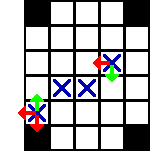
\includegraphics{imgs/verifDepl}
\end{figure}
		
\subsubsection{Détection}	
	
Pour pouvoir détecter toutes les cases à détruire, nous utilisons une autre grille de la même taille que celle contenant les éléments, mais cette nouvelle grille contient des booléens. Chaque case est ainsi associée à un booléen. Si la case doit être détruite, le booléens vaudra vrai.

On va ensuite parcourir la première grille ligne par ligne pour marquer tous les alignements horizontaux puis colonne par colonne pour les combinaisons verticales.

\begin{figure}[position]
	\center
	\caption{\label{Detection} Détection}
	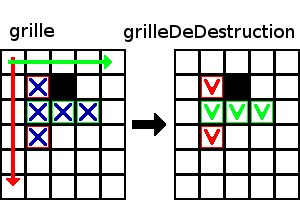
\includegraphics{imgs/Detection}
\end{figure}

Nous avons besoin de quelques nouvelles variables :

\begin{lstlisting}
int couleurTemp; // Couleur temporaire qui va servir pour verifier que plusieurs cases sont identiques
int nbCasesAlignees; // Sert a compter le nombre de cases alignees
\end{lstlisting}

Pour parcourir la grille :

\begin{lstlisting}
for(int j = 0; j < tailleGrilleY; j++)
{
	couleurTemp = grille[0][j]; // La couleur temporaire est egale a la premiere case de la grille
	nbCasesAlignees = 1; // Le nombre de cases alignees est egal a 1 en debut de ligne
	/** Parcours des lignes **/
	for(int i = 0; i < tailleGrilleX; i++)
	{
		if(couleurTemp == grille[i][j]) // Si la couleur temporaire est la meme dans cette case, on incremente nbCasesAlignees
			nbCasesAlignees++;
		else if(nbCasesAlignees >= 3)
		{
			// Si la couleur n'est pas la meme mais qu'on a un alignement, on note dans le deuxieme tableau
			nbCasesAlignees = 1;
			couleurTemp = grille[i][j];
			pasDeCasesADetruire = false;
		}
		else
		{
			nbCasesAlignees = 1;
			couleurTemp = grille[i][j];
		}

		if(i == tailleGrilleX - 1 && nbCasesAlignees >= 3) 
			/* Si on atteind le bord de la grille et qu'on a un alignement de plus de 3,
			on note dans le tableau apres avoir incremente i, pour utiliser la meme fonction de notation dans l'autre tableau. */
	}
} 
\end{lstlisting}
		Pour noter les cases à détruire dans la seconde grille, on peut simplement faire :
\begin{lstlisting}
for(int k = i - nbCasesAlignees; k < i; k++) // On parcours les cases a noter, mais on ne passe pas quand k == i car la case i ne fait pas partie de l'alignement
{
	grilleDeDestruction[k][j] = true;
}
\end{lstlisting}

Il faudra refaire ce processus de détection des alignements verticalement, donc colonne par colonne. Le principe est identique.

\subsubsection{Destruction}

Pour détruire les cases, nous remplaçons les cases à détruire par -1 dans la grille.

\begin{figure}[position]
	\center
	\caption{\label{Destruction} Destruction}
	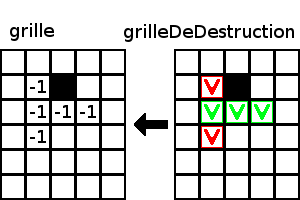
\includegraphics{imgs/Destruction}
\end{figure}

Cela se traduit comme suit :

\begin{lstlisting}
for(int j = 0; j < tailleGrilleY; j++)
{
	for(int i = 0; i < tailleGrilleX; i++)
	{
		if(grilleDeDestruction[i][j] == true)
		{
			grille[i][j] = -1;
			grilleDeDestruction[i][j] = false; // On en profite pour reinitialiser la deuxieme grille qui sert pour la destruction
		}
	}
}
\end{lstlisting}

\subsubsection{Remplacement}

	Afin de remplacer les cases détruites (donc -1 dans la grille), il faut trier la grille de manière à avoir tout les -1 au dessus.
	Il faut tout de même penser aux cases inutilisables (0 dans la grille) qui ne doivent pas être bougées.
	
	Nous allons donc parcourir chaque colonne en partant du bas, et lorsqu'on trouve un -1, nous allons le remplacer par la prochaine case valide (qu'on mettra à -1).
	
\begin{figure}[position]
	\center
	\caption{\label{Remplacement} Remplacement}
	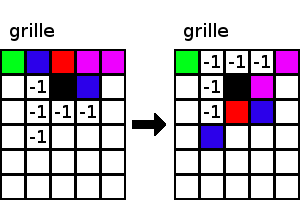
\includegraphics{imgs/Remplacement1}
	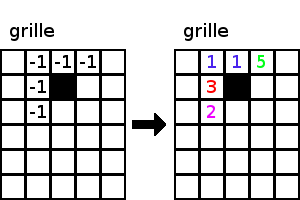
\includegraphics{imgs/Remplacement2}
\end{figure}
	
	Pour une colonne k, nous aurons :
\begin{lstlisting}
int j;
boolean continuer;
for(int i = tailleGrilleY - 1; i >= 0; i--)
{
	if(grille[k][j] == -1)
	{
		j = i;
		continuer = true;
		while(j >= 0 && continuer == true)
		{
			j--;
			if(grille[k][j] != 0 && grille[k][j] != -1) // Si on trouve une case correcte, on remplace
			{
				grille[k][i] = grille[k][j];
				grille[k][j] = -1;
				continuer = false; // On n'a plus besoin de rechercher
			}
		}
	}
}
\end{lstlisting}

	Il faudra faire une boucle pour répliquer ce résonnement à chaque colonne. Notons qu'on pourrais ajouter une condition qui arrêterais la boucle la première fois que le while ne trouve pas de case valide.
	
	Désormais, il ne reste plus qu'à remplacer toutes les cases -1 par un numéro aléatoire 1, 2, 3, 4 ou 5 représentant les différents types de cases.

\begin{lstlisting}
for(int j = 0; j < tailleGrilleY; j++)
{
	for(int i = 0; i < tailleGrilleX; i++)
	{
		if(grille[i][j] == -1;
			grille[i][j] = (int)(Math.random() * 5) + 1;
	}
}
\end{lstlisting}

\subsubsection{Finalement}

Ce processus Détection-Destruction-Remplacement devra être répété jusqu'à ce qu'il n'y ait plus aucune case à détruire.

De plus, un score à atteindre pourra être fixé. Pour cela, chaque destruction de case (quand on les mets à -1) incrémentera d'un certain nombre de points la variable scoreActuel. Le jeu pourra s'arrêter lorsque le score ciblé est atteint.
\begin{lstlisting}
scoreActuel >= scoreCible
\end{lstlisting}

Il est également possible de compter le nombre de coups que le joueur a utilisé. En effet, il suffit de le faire lors de l'échangement des cases. Si cet échange est par la suite annulé, le nombre de coups sera remis à son état d'avant l'échange.
Avec ceci, on peut définir un certain nombre de vies que le joueur possède, et qu'il perd à la perte d'un niveau, quand il n'a plus de vie, il doit attendre pour pouvoir continuer à jouer.
Enfin, lors du premier remplissage de la grille (un nombre aléatoire dans chaque case), il faudra éliminer toutes le combinaisons, c'est à dire lancer le processus Détection-Destruction-Remplacement autant de fois qu'il le faudra.

\subsection{Annexe}
Dans cette partie, nous ajouterons les analyses que nous avons pu faire sur \emph{Candy Crush} mais qui sont difficilement réalisables.
On peut compter parmi celles-ci les bonus qui s'obtiennent par certaines combinaisons de bonbons.
\begin{itemize}

\item
	Combinaison de 4 bonbons = un bonbon spécial qui détruit une ligne ou une colonne entière (selon le sens de ses rayures)

\item
	Combinaison de 5 bonbons = bombe multicolore (l'associer avec un autre bonbon détruit tout les bonbons du type associé présents dans la grille)
\item
	Bonbons spéciaux qui détruisent tout les bonbons autour d'eux : quand on fait deux combinaisons de 3 (en L)
\item
	Bonbons à retardement : vont exploser et détruire les bonbons autour d'eux 
\item
	Association de deux bonbons spéciaux pour un plus gros (détruit 3 lignes et 3 colonnes)      
\item
	Combos : une combinaison en entraîne d'autres (ajout de points)
\item
	Une combinaison détruit les bonbons et d'autres les remplacent (tombent du dessus) 
\item
	Destruction automatique des bonbons spéciaux à la fin du niveau

\end{itemize}


\section{Jeu 2 : Centipede}
\documentclass[a4paper, 12pt, twoside]{article}

\usepackage[utf8]{inputenc}
\usepackage[T1]{fontenc}
\usepackage{lmodern} % Enlève plein de warnings :D et permet le tt gras
\usepackage[french]{babel}

% \usepackage[usenames,dvipsnames,svgnames,table]{xcolor}

\usepackage{amsmath}
\usepackage{amssymb}
% \usepackage{mathrsfs}

\usepackage{scrextend}

\usepackage{color}
\usepackage{listings}
\definecolor{listinggray}{gray}{0.9}
\definecolor{lbcolor}{rgb}{0.95,0.95,0.95}
\lstset{
	backgroundcolor=\color{lbcolor},
	tabsize=4,
	rulecolor=,
	language=Java,
	basicstyle=\small\ttfamily,
	upquote=false,
	aboveskip={.5\baselineskip},
	columns=fixed,
	showstringspaces=false,
	extendedchars=true,
	showspaces=false,
	breaklines=true,
	prebreak = \raisebox{0ex}[0ex][0ex]{\ensuremath{\hookleftarrow}},
	frame=single,
	showtabs=false,
	identifierstyle=\ttfamily,
	keywordstyle=\bfseries\color[rgb]{0,0,1},
	commentstyle=\color[rgb]{0.133,0.545,0.133},
	stringstyle=\color[rgb]{0.627,0.126,0.941},
}

% ---------------
% Commmandes
% ---------------

% Argument obligatoire : nom du type agrégé
\newenvironment{typeag}[1][]{\noindent \textbf{type} \texttt{#1} \{\begin{addmargin}[2em]{0em}}{\end{addmargin}\}}
% Arguments obligatoires : Nom — Type — Description
\newcommand{\variable}[3]{\noindent \texttt{#1} : \textit{#2} --- #3}

% \renewcommand\arraystretch{1.2}

% ---------------
% Main
% ---------------
\title{Projet d'Initiation à l'Ingénierie Logicielle\\Rapport groupe \no 3}
\author{Mohammed \bsc{Lakal}\\Émile \bsc{Jeannin}\\Théo \bsc{Mottet}\\Alexis \bsc{Cabodi}}
\date{Révision du\\\today}

\begin{document}
\maketitle
\newpage
\tableofcontents
\newpage
\section{Jeu 1 : Candy Crush}
\section{Introduction}

Centipède est un jeu développé par Atari Inc, sorti en 1981. Ce jeu à été réalisé par Dona Bailey et Ed Logg. Centipede est considéré comme le premier jeu à avoir attiré des femmes dans les salles d'arcades. 
Le joueur se défend contre les centipèdes, les araignées , les scorpions et les puces. Le joueur gagne un round après avoir éliminé le centipede qui serpente entre les champignons. Actuellement le record du monde de centipede en terme de score est de 7 111 111 points. Celui-ci est détenu par Donald Hayes qui à réalisé se record le 5 novembre 2000. 
C'est pourquoi, dans le cadre du projet ingénierie logiciel nous allons analyser ce jeu, cela nous apportera une première approche du monde de la création de jeu vidéo et du développement d'un tel jeu. 
\section{Jeu 2 : Centipede}
\subsection{État du jeu}

Dans cette partie nous traiterons l'état du jeu "Centipede". Au début du jeu : 
vous avez un personnage : 

\begin{typeag}[Personnage]
        \variable{vies}{entier}{Nombre de vies du personnage}\\
        \variable{positionX}{entier}{Abcisse du personnage sur la zone}\\
        \variable{positionY}{entier}{Ordonnée du personnage sur la zone}
\end{typeag}

une zone de jeu composé de différents éléments : 

\begin{typeag}[Zone de jeu]
        \variable{grille}{Champignon c [ligne][colonne]}{représente l'ensemble des cases avec un champignon ou non}\\
        \variable{couleurs}{entier}{indique le jeu de couleurs du niveau actuel}\\
        \variable{score}{entier}{nombre qui représente le score du joueur en temps réel}\\
        \variable{tir}{}{représente le tir unique que possède le joueur}
        \variable{niveau}{entier}{compteur de niveau}
\end{typeag}

où  sont aussi disposés des champignons, à noter que ces champignons sont disposés aléatoirement sur la grille, de même que leur nombre. 

Les champignons sont représentés par :

\begin{typeag}[Champignon c]
        \variable{vie}{entier}{de 0 (pas de champignon) à 4 (champignon "neuf")}\\
        \variable{vénéneux}{booléen}{indique si le champignon est vénéneux ou pas}\\
        \variable{positionX}{entier}{Abcisse du champignon sur la zone de jeu}\\
        \variable{positionY}{entier}{Ordonnée du champignon sur la zone de jeu}
\end{typeag}

Au départ, il y a aussi un ennemi, le centipede : 
Celui-ci est représenté comme cela : 

\begin{typeag}[Segment ( 12 segments représentent le centipede)]
        \variable{état}{entier}{prend la valeur : 0 si le centipede est mort, 1 si le centipede est une tête seule, 2 si le centipede est complet au niveau de ses 12 segments}\\
        \variable{vitesse}{entier}{indique la vitesse du centipede en fonction du niveau où se trouve le joueur}\\
        \variable{donnée}{entier}{si estTête respectivement 0,1,2,3 pour haut,bas,gauche,droite, sinon indique quel segment il suit}
        \variable{positionX}{entier}{Abcisse du centipede sur la zone de jeu}\\
        \variable{positionY}{entier}{Ordonnée du centipede sur la zone de jeu}
\end{typeag}

Pour contrer le centipede le joueur dispose d'un tir unique.
Le tir est représenté comme cela : 

\begin{typeag}[un tir unique]
        \variable{booléen}{actif}{indique si le projectile est actuellement en mouvement ou prêt à être relancé}\\
        \variable{vitesse}{entier}{indique la vitesse du tir : celui-ci a toujours la même vitesse dans tous les niveaux}\\
        \variable{positionX}{entier ou réel}{Abcisse du tir sur la zone de jeu}\\
        \variable{positionY}{entier ou réel}{Ordonnée du tir sur la zone de jeu}
\end{typeag}

Néanmoins le joueur ne doit pas vaincre uniquement le centipede, d'autres ennemis apparaissent au fur et à mesure des niveaux que le joueur passe : 
Ceux ci sont répresnté dans une variable ennemi : 

\begin{typeag}[Ennemi]
        \variable{type}{entier}{indique le type d'ennemi en face du joueur : 0 = araignée ; 1 = puce ; 2 = scorpion}\\
        \variable{vitesse}{entier}{indique la vitesse de l'ennemi qui est différente en fonction du niveau joué et du score du joueur}\\
        \variable{positionX}{entier ou réel}{Abcisse de ou des ennemis sur la zone de jeu}\\
        \variable{positionY}{entier ou réel}{Ordonnée du tir sur la zone de jeu}
\end{typeag}


\subsection{Configuration initiale du jeu}
Dans cette seconde partie nous allons traiter la situation de départ du jeu. Dès le lancement du jeu le joueur dispose d'un certain nombre d'éléments : 

\begin{itemize}
\item 
	Le joueur dispose d'un compteur de point : son score qui se situe en haut à gauche de son écran de jeu. Celui ci au départ est égal à 0.
	\item 
	Le joueur dispose peut également visualiser son score "record" en haut au milieu de son écran de jeu. De cette manière il sait quel score il doit atteindre pour s'améliorer.
	\item
	Le joueur peut également visualiser le nombre de vie qu'il possède et qu'il lui reste à utiliser. Celle-ci sont représentées par une tête de lutin, chacune de ces têtes sont situées à coté du score du joueur.
\end{itemize}


Ensuite à chaque début de partie, le joueur à devant lui, sur la  \itshape{Zone de jeu} : 

\begin{itemize}
	\item
	Un certain nombre de champignon réparties aléatoirement en nombre et en position sur la  \itshape{Zone de jeu}
	\item
	Le centipede, ennemi du joueur, composé de \itshape{Segments} au nombre de 12. Ils sont d'abord de taille 1, et évoluerons par la suite jusqu'à leurs tailles maximales. Le centipede arrive dans la partie depuis le haut de la \itshape{Zone de jeu}, et au milieu de celle ci. 
\end{itemize}
 



\subsection{Évolution de l'état du jeu}

Dans cette partie nous allons étudier les points d'interaction du jeu avec le joueur, leurs conséquences sur le jeu ainsi que l'évolution automatique de l'état du jeu. 
Le jeu va tourner en boucle jusqu'à ce que l'on perde toutes nos vies et que le score bonus ne nous en redonne pas :
\begin{lstlisting}
while ( personnage.vies > 0 ) {
	// Recuperation des entrees
	// Traitement et declenchement des sons
	// Affichage a l'ecran
}
\end{lstlisting}
Dans un premier temps, le joueur peut se déplacer soit grâce au flèche du clavier, soit avec la souris. De plus, le joueur afin de se défendre des ennemis à la possibilité de tirer un projectile avec la touche espace, ou le clic gauche de la souris. Or il ne peut le faire que si le projectile n'est pas à l'écran. En effet, il ne peut y avoir qu'un seul projectile sur l'écran, c'est pourquoi le tire est unique. Cependant le joueur peut tout de même afin de se défendre, éviter l'ennemi mais en aucun cas, le joueur ne pourra gagner s'il ne tire pas et ne détruit pas l'ennemi, si le joueur est tenté de faire ça ( toujours éviter l'ennemi, alors, la partie sera infinie. Le joueur restera toujours bloqué au même niveau. De plus, si le joueur rentre en contact avec un des ennemi, alors le joueur ce verra perdre une vie et il meurt. Si le joueur possède encore une vie, alors le niveau recommencera, cependant le niveau précédent se verra perdre les champignons rendu vénéneux qui seront donc ajouté au score du joueur mais le nouveau niveau lui sera pourvu de plus de champignons que le niveau précédent. 
Concernant le projectile que peut tirer l'auteur,comme dit plus haut, celui-ci est unique. Si le projectile tiré touche un ennemi, rentre en contact avec un ennemi alors l'ennemi meurt et le joueur gagne alors des points en fonction de l'ennemi tué. Si le joueur tue une partie du corps du centipede, celle ci se transforme alors en champignon sur la position de sa mort et rapporte au joueur 10 points. Si le joueur touche la tête du centipede alors il gagne 100 points et transforme la tête du centipede en champignon. Si le joueur tue une araignée, celui peut être récompensé en fonction des risques qu'il a pris pour tuer celle-ci, en effet, si le joueur tue l'araignée à une distance très proche de celle-ci alors il gagnera 900 points, à une distance moyenne il gagnera 600 points, et a une distance éloignée il gagnera 300 points. Le joueur peut également tué les champignons qui possède chacun, 4 points de vie, il faut donc 4 tirs de la part du joueur afin de tuer un champignon. De plus les champignons ont une certaines visées stratégiques, car l'utilisateur peut les utiliser pour diriger le centipede la ou il le veut et donc le tuer plus facilement. Le joueur peut tué le scorpion qui rend les champignons vénéneux, si le joueur y arrive alors il est récompensé par 1000 points. Le joueur peut aussi tué une puce, ce qui lui rapporte 200 points. Cette puce apparait que dans un certain cas particulier, en effet elle apparait seulement si il y a moins de 5 champignons dans la zone de déplacement du joueur elle apparaît aléatoirement en une position x et  descend jusqu'en bas du tableau, en déposant des champignons aléatoirement en y.  De plus, un scorpion apparait aléatoirement à partir d'un certain niveau et se déplace sur une ligne en rendant les champignons vénéneux. Dès lors si le centipede touche un des champignons vénéneux alors celui-ci descendra en ligne droite jusqu'à la zone du joueur. Ce qui rend le jeu encore plus difficile et hardu.

\section{Conclusion}

Afin de conclure, nous pouvons dire que centipede est un jeu d'une difficulté extrême, qui demande beaucoup d'entrainement  et beaucoup de réflexion. En effet, le jeu demande à l'utilisateur de comprendre les mécanismes du centipede, des ennemis et de gérer les évènements aléatoires tels que les scorpions. De plus, le jeu demande l'adoption d'une certaine stratégie si l'utilisateur veut progresser plus loin et atteindre un score vraiment élevé, en effet, il peut créer des endroits dit " safe " ou alors créer des couloirs pour pouvoir tuer aisément le centipede. En tout point, ce jeu est donc aussi complexe que Candy Crush, en effet, celui-ci demande de la réflexion afin de réaliser de meilleur score. L'utilisateur doit anticiper les déplacements des bonbons afin de créer des combinaisons a 4 ou 5 bonbons. L'utilisateur doit aussi comprendre les mécanismes du jeu dans des niveaux ou les objectifs sont d'éliminer la gélatine, ou de faire tomber des ingrédients... L'utilisateur doit constamment rechercher les meilleurs combinaisons... 

Nous pouvons donc dire que ces deux jeux peuvent permettre à l'utilisateur de développer ses capacités de réflexion et d'adaptation.

\end{document}

\section{Conclusion}
Afin de conclure, nous pouvons dire que Centipede est un jeu d'une difficulté extrême, qui demande beaucoup d'entraînement et beaucoup de réflexion. En effet, le jeu demande à l'utilisateur de comprendre les mécanismes du centipède, des ennemis et de gérer les événements aléatoires tels que les scorpions. De plus, le jeu demande l'adoption d'une certaine stratégie si l'utilisateur veut progresser plus loin et atteindre un score vraiment élevé. En effet, il peut créer des endroits dits " safe " ou alors créer des couloirs pour pouvoir tuer aisément le centipède. En tout point, ce jeu est donc aussi complexe que Candy Crush. En effet, celui-ci demande de la réflexion afin de réaliser de meilleurs scores. L'utilisateur doit anticiper les déplacements des bonbons afin de créer des combinaisons a 4 ou 5 bonbons. L'utilisateur doit aussi comprendre les mécanismes du jeu dans des niveaux où les objectifs sont d'éliminer la gélatine, ou de faire tomber des ingrédients... L'utilisateur doit constamment rechercher les meilleurs combinaisons... 

Nous pouvons donc dire que ces deux jeux peuvent permettre à l'utilisateur de développer ses capacités de réflexion et d'adaptation.

\end{document}
